\documentclass[tikz]{standalone}
\usepackage{tikz}
\usetikzlibrary{positioning}


\begin{document}
	
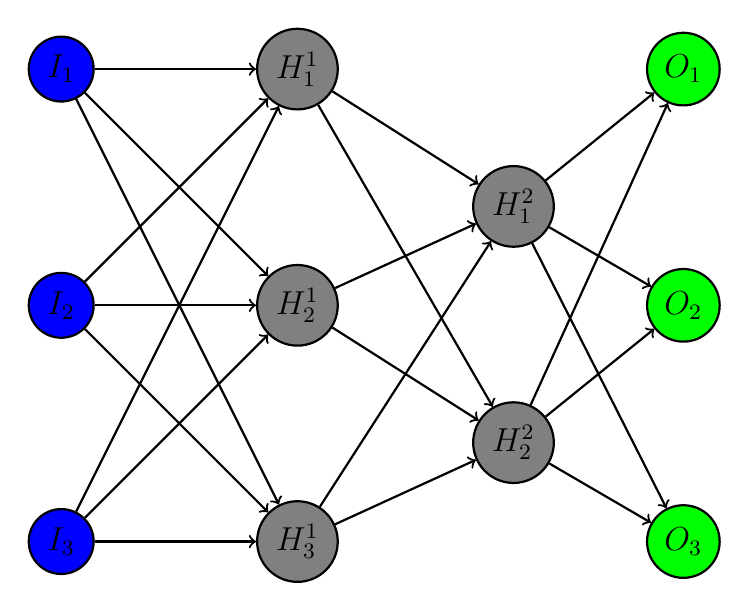
\begin{tikzpicture}[auto, node distance=3cm, every loop/.style={},
thick,main node/.style={circle,draw,font=\sffamily\large\bfseries}]

\node[main node] [fill=blue] (A) {$I_1$};
\node[main node] [fill=blue] (B) [below of=A] {$I_2$};
\node[main node] [fill=blue] (C) [below of=B] {$I_3$};
\node[main node] [fill=gray] (D) [right of=A] {$H^1_1$};
\node[main node] [fill=gray] (E) [right of=B] {$H^1_2$};
\node[main node] [fill=gray] (F) [right of=C] {$H^1_3$};
\node[main node] [fill=gray] (G) [below right = 1cm and 2cm of D] {$H^2_1$};
\node[main node] [fill=gray] (H) [below right = 1cm and 2cm of E] {$H^2_2$};
\node[main node] [fill=green] (I) [right = 7cm of A] {$O_1$};
\node[main node] [fill=green] (J) [right = 7cm of B] {$O_2$};
\node[main node] [fill=green] (K) [right = 7cm of C] {$O_3$};

\foreach \x in {D,E,F}
\path[every node/.style={font=\sffamily\normalsize}]
(A) [->] edge node [] {} (\x)
(B) [->] edge node [] {} (\x)
(C) [->] edge node [] {} (\x);
\foreach \x in {G,H}
\path[every node/.style={font=\sffamily\normalsize}]
(D) [->] edge node [] {} (\x)
(E) [->] edge node [] {} (\x)
(F) [->] edge node [] {} (\x);
\foreach \x in {I,J,K}
\path[every node/.style={font=\sffamily\normalsize}]
(G) [->] edge node [] {} (\x)
(H) [->] edge node [] {} (\x);
\end{tikzpicture}


\end{document}